\input{../header}
\hyphenpenalty=5000

\rhead{Your name: \rule{8cm}{0.15mm}}

\begin{document}

\everymath{\displaystyle}

\section{Learning target A5, version 1}

Use definite integrals to compute physical quantities, such as work, force, pressure, energy, etc.



\hrulefill

Consider a trough with a triangular end as pictured below. The trough is 12 feet wide along its top, 15 feet deep, 18 feet long, and it is full of water to a depth of 13 feet.   As usual, the weight density of water is 62.4 pounds per cubic foot.

\begin{enumerate}[leftmargin=15pt]

	\item \emph{Determine the total amount of hydrostatic force on one end of the trough}.  Clearly show relevant slices that go in to determining the definite integral that answers the question. State the appropriate definite integral clearly and evaluate it using technology to determine the total force.  Include units on your result.

\hfill \scalebox{0.4}{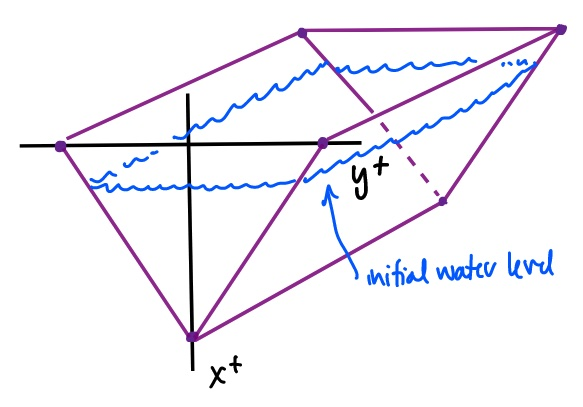
\includegraphics{images/LT-8-tank-3}}

\vfill

	\item \emph{Determine the total amount of work that would be required to empty the trough until 3 feet of water remains in it, while pumping the water to a truck whose tank is 6 feet above the top of the trough}.  Clearly show the relevant slice(s) and computations that are involved in determining the definite integral that answers the question.  State the appropriate definite integral clearly and evaluate it using technology to determine the total work.  Include units on your result.
	
\hfill \scalebox{0.4}{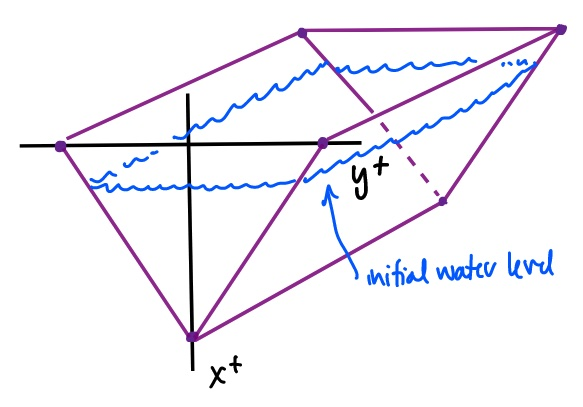
\includegraphics{images/LT-8-tank-3}}

\vfill

\end{enumerate}
	
%%%%%%%%%%%%%%%%%%%%%%%%%%%%%%%%%%%%%%%%%%%%%%%%%%%%%%%%%%%%%%%
\pagebreak
\section{Learning target A5, version 2}

Use definite integrals to compute physical quantities, such as work, force, pressure, energy, etc.

\hrulefill

Some asshole in a calculus problem constructed a trapezoidal fish tank as pictured below. The fish tank is 1.5 feet across the top, 2 feet across the bottom, 2 feet tall, and 3 feet long, and it's filled to a depth of 1.75 feet of water. 
As usual, the weight density of water is 62.4 pounds per cubic foot.

\begin{enumerate}[(a), leftmargin=15pt]

	\item \emph{Determine the total amount of hydrostatic force on one of the flat ends of the tank}. \\
	Draw a slice, label it carefully, and show your work to write down the appropriate definite integral.
	Remember, in American units, pressure is 62.4 times water depth.

\hfill \scalebox{0.5}{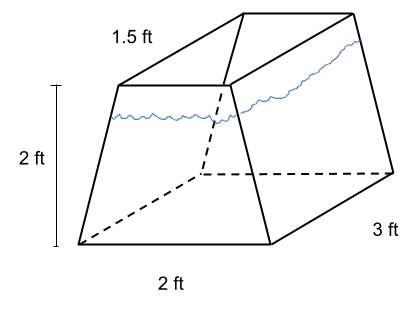
\includegraphics{images/trapezoid-tank}}

\vfill

	\item \emph{Find the total amount of work that would be required to pump all the water out of the tank}.  \\
	Draw a slice, label it carefully, and show your work to write down the appropriate definite integral. Remember, in American units, ``pounds'' is a force.
	
\hfill \scalebox{0.5}{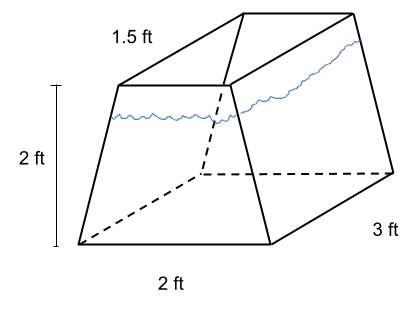
\includegraphics{images/trapezoid-tank}}

\vfill

\end{enumerate}
%%%%%%%%%%%%%%%%%%%%%%%%%%%%%%%%%%%%%%%%%%%%%%%%%%%%%%%%%%%%%%%
\pagebreak
\section{Learning target A5, version 3}

Use definite integrals to compute physical quantities, such as work, force, pressure, energy, etc.

\hrulefill

Consider a trough with a trapezoidal end as pictured below. Assume the trough is 14 feet wide along its top, 12 feet wide along its bottom, 7 feet deep, 20 feet long, and that it is full of water to a depth of 6 feet.   As usual, the weight density of water is 62.4 pounds per cubic foot.

\begin{enumerate}[(a), leftmargin=15pt]

	\item \emph{Determine the total amount of hydrostatic force on one of the flat ends of the tank}. \\
	Draw a slice, label it carefully, and show your work to write down the appropriate definite integral.
	Remember, in American units, pressure is 62.4 times water depth.

\hfill \scalebox{0.5}{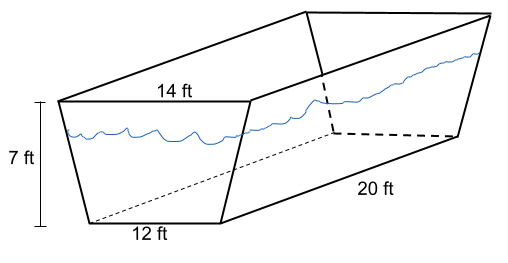
\includegraphics{images/trapezoid-trough}}

\vfill

	\item \emph{Find the total amount of work that would be required to pump all the water out of the tank}.  \\
	Draw a slice, label it carefully, and show your work to write down the appropriate definite integral. Remember, in American units, ``pounds'' is a force.
	
\hfill \scalebox{0.5}{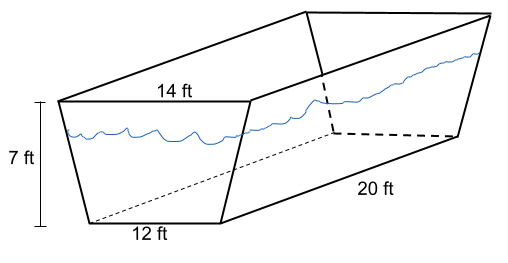
\includegraphics{images/trapezoid-trough}}

\vfill

\end{enumerate}
%%%%%%%%%%%%%%%%%%%%%%%%%%%%%%%%%%%%%%%%%%%%%%%%%%%%%%%%%%%%%%%
\pagebreak

%%%%%%%%%%%%%%%%%%%%%%%%%%%%%%%%%%%%%%%%%%%%%%%%%%%%%%%%%%%%%%%
\pagebreak
\renewcommand{\thefootnote}{\fnsymbol{footnote}}
\setlength{\skip\footins}{2cm}
\section{Learning target A5, version 4}

Use definite integrals to compute physical quantities, such as work, force, pressure, energy, etc.

\hrulefill

Evidence suggests that the Great Pyramid of Giza was originally constructed to serve as a fish tank for a colossal and now extinct species of fish called ``abtu.''*\marginpar{\tiny * This is not true.} Let us consider the amount of work that would have been required to remove the 450 feet of water from the fish tank when the ancient Egyptians decided to turn it into a burial monument instead.

\begin{center}
	\scalebox{0.5}{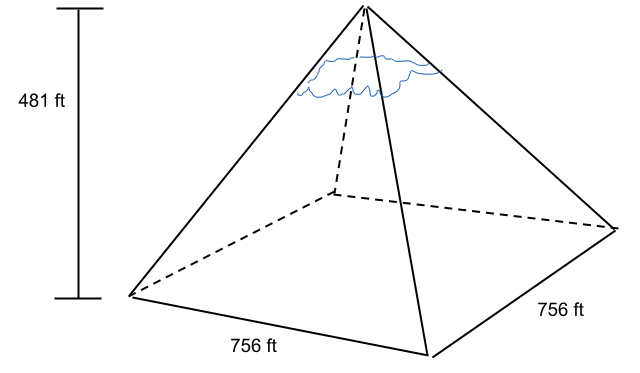
\includegraphics{images/pyramid}}
\end{center}

\begin{enumerate}[(a), leftmargin=15pt]

	\item We need to slice the water horizontally into thin square slabs. Draw a representative slice.
	\item We need a letter to represent the position of this slice. There are several ways to do this: we could measure down from the peak of the pyramid, we could measure up from the base of the pyramid, or we could even measure down from the water level. Choose one of these ways, \textbf{draw a line from your reference level to the slice,} and label this line with a letter.
	\item We need to write down the \textbf{width} of the slice, and the \textbf{distance to lift} each slice, as functions of our new letter. Fill in the following tables; start by putting your letter inside the parentheses.

	\begin{minipage}{0.45\textwidth}
		\scalebox{0.85}{\begin{tabular}{c|c|c}
		location         & top of pyramid & base of pyramid  \\\hline
		\Big(\qquad \Big) & \phantom{$\displaystyle\int$}       &                  \\\hline
		width            & 0              & 756             
		\end{tabular}}
	\end{minipage}
	\begin{minipage}{0.45\textwidth}
		\scalebox{0.85}{\begin{tabular}{c|c|c}
		location         & top of pyramid & base of pyramid  \\\hline
		\Big(\qquad \Big) & \phantom{$\displaystyle\int$}       &                  \\\hline
		distance to lift            & 0              & 481             
		\end{tabular}}
	\end{minipage}
	\item Use the tables above to write down equations for the width of the slice and the distance to lift each slice as a function of your new letter. (If I were you, I'd use point-slope form.)
	\vfill
	Turn the page over now please :)
	\pagebreak

	\begin{center}
		\scalebox{0.5}{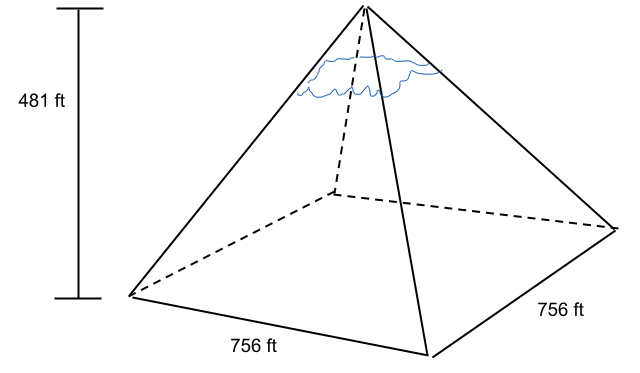
\includegraphics{images/pyramid}}
	\end{center}

	\item Remember how I said there were \textbf{several} ways to do this? Choose a \textbf{different} way, draw a \textbf{different} line, and label it with a \textbf{different} letter.
	\item Same deal with tables and equations.

	\begin{minipage}{0.45\textwidth}
		\scalebox{0.85}{\begin{tabular}{c|c|c}
		location         & top of pyramid & base of pyramid  \\\hline
		\Big(\qquad \Big) & \phantom{$\displaystyle\int$}       &                  \\\hline
		width            & 0              & 756             
		\end{tabular}}
	\end{minipage}
	\begin{minipage}{0.45\textwidth}
		\scalebox{0.85}{\begin{tabular}{c|c|c}
		location         & top of pyramid & base of pyramid  \\\hline
		\Big(\qquad \Big) & \phantom{$\displaystyle\int$}       &                  \\\hline
		distance to lift            & 0              & 481             
		\end{tabular}}
	\end{minipage}
	\vfill
	\item Write down $\Delta W$, the amount of work done to lift a slice, using your first letter. \\
	{\small Some reminders: $W = F \cdot D$, ``pounds'' is a force unit, and the weight density of water is 62.4 lbs / ft$^3$.}
	\vfill
	\item Using your first letter, write down a definite integral that computes the total amount of work.
	\vfill
	\item Repeat the prior two steps using your second letter.
	\vfill
	

\end{enumerate}

\end{document}